\chapter{Oerba 200AF}

%This shoudl all be done with actual figures

Anomaly 1 - Stage 1

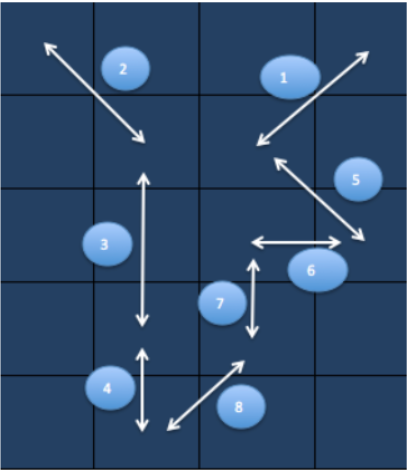
\includegraphics{Images/anomaly1stage1}

\pickup{2 Ghysal Greens}{on the right if possible without getting an encounter}

Anomaly 2 - Stage 1

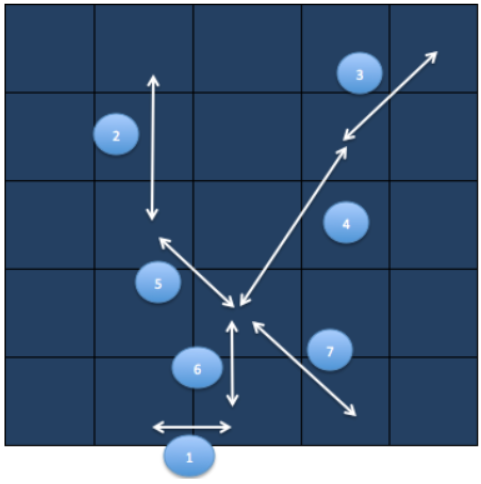
\includegraphics{Images/anomaly2stage1}

Anomaly 2 - Stage 2

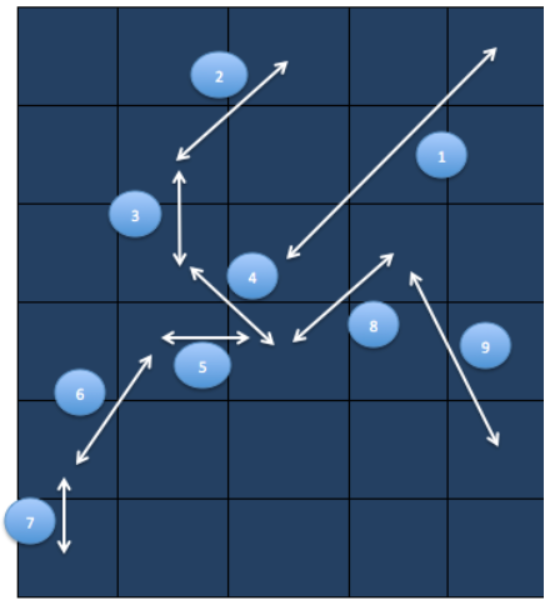
\includegraphics{Images/anomaly2stage2}

\pickup{500 Gil}{near the tree}

Anomaly 3 - Stage 1

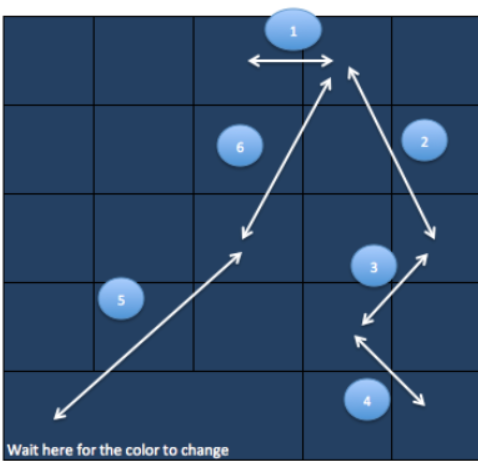
\includegraphics{Images/anomaly3stage1}

Anomaly 3 - Stage 2

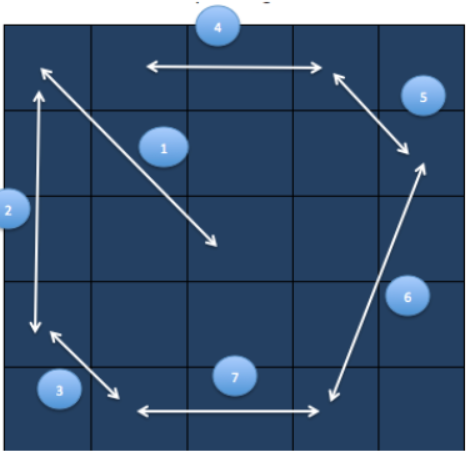
\includegraphics{Images/anomaly3stage2}

Anomaly 3 - Stage 3

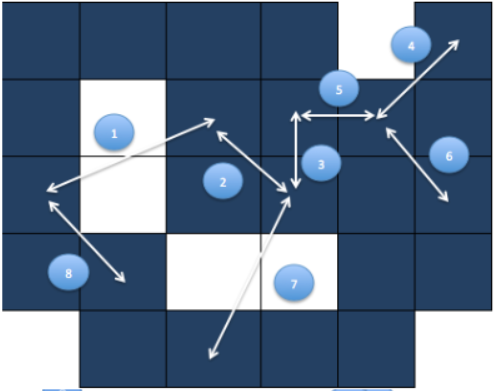
\includegraphics{images/anomaly3stage3}

\begin{menu}
	\begin{itemize}
		\crystarium
		\begin{itemize}
			\item Noel:
			      \begin{itemize}
				      \item All \rav
				      \item \stagebonus{\rav}
			      \end{itemize}
			\item Serah:
			      \begin{itemize}
				      \item All \rav
				      \item \stagebonus{ATB Level}
			      \end{itemize}
		\end{itemize}
	\end{itemize}
\end{menu}

\pickup{Librascope}{at the stairs}

\pickup{600 Gil}{in the house}

\begin{battle}{Oerba Caius}
	\begin{itemize}
		\item \sixth
		      \begin{itemize}
			      \item Shift
		      \end{itemize}
		\item \second
		      \begin{itemize}
			      \item Auto-Chain
			      \item Gahongas Feral Link, \circlec, \squarec, \circlec
		      \end{itemize}
		\item \third
		      \begin{itemize}
			      \item Auto-Chain
		      \end{itemize}
		\item \fifth
		      \begin{itemize}
			      \item Blizzara-Aerora
			      \item Repeat, \com-buffer into
		      \end{itemize}
		\item \first
		      \begin{itemize}
			      \item Ruins x dead
		      \end{itemize}
	\end{itemize}
\end{battle}

\pickup{Artifact of Origins}{in front of you}. Force an encounter in the corner wall. Get on the Chocobo. Get the Ghysal Greens and Librascope if you haven't already. \pickup{hidden Graviton Core}{on the schoolhouse roof} Head to the gate.
\newline